\subsection*{3 a)}
\textbf{Finn divergensen $\nabla \cdot \textbf{v} = \partial v_x /\partial x
+  \partial v_y /\partial y$ og virvlingen $\nabla \cross \textbf{v} =
\left(\partial v_y /\partial x - \partial v_x /\partial y\right)\textbf{k}$
av hastighetsfeltet.}
\\
\\
Vi får oppgitt:

\begin{align*}
    v_x = \cos(x)\sin(y), \qquad v_y = - \sin(x)\cos(y)
    \\
\end{align*}

Det gir at divergensen, $\nabla \cdot \textbf{v} = \partial v_x /\partial x
+  \partial v_y /\partial y$, er lik:

\begin{align*}
    \frac{\partial v_x}{\partial x}
    +
    \frac{\partial v_y}{\partial y}
    &=
    \frac{\partial \cos(x)\sin(y)}{\partial x}
    +
    \frac{\partial - \sin(x)\cos(y)}{\partial y}
    \\
    \\
    \frac{\partial \cos(x)\sin(y)}{\partial x}
    =
     -\sin(x)\sin(y)
    &\qquad \qquad
    \frac{\partial - \sin(x)\cos(y)}{\partial y}
    =
    \sin(x)\sin(y)
    \\
    \\
    \nabla \cdot \textbf{v} &= \sin(x)\sin(y) - \sin(x)\sin(y)
    = \underline{\underline{0}}
    \\
    \\
\end{align*}

Videre kan vi finne virvlingen, $\nabla \cross \textbf{v} =
(\partial v_y /\partial x+  \partial v_x /\partial y) \textbf{k}$:


\begin{align*}
    \left(\frac{\partial v_y}{\partial x}
    -
    \frac{\partial v_x}{\partial y}\right) \textbf{k}
    &=
    \left(\frac{\partial -\sin(x)\cos(y)}{\partial x}
    -
    \frac{\partial \cos(x)\sin(y)}{\partial y}\right) \textbf{k}
    \\
    \\
    \frac{\partial - \sin(x)\cos(y)}{\partial x}
    =
     -\cos(x)\cos(y)
    &\qquad \qquad
    \frac{\partial \cos(x)\sin(y)}{\partial y}
    =
    \cos(x) \cos(y)
    \\
    \\
    \nabla \cross \textbf{v}
    &=
    -\cos(x)\cos(y) - \cos(x)\cos(y)\textbf{k}
    =
    \underline{\underline{-2\cos(x)\cos(y)\textbf{k}}}
\end{align*}










\pagebreak
\subsection*{3 b)}
\textbf{Tegn opp strømvektorer langs x- og y-aksen.}
\\
\\
\begin{figure}[H]
		\centering
		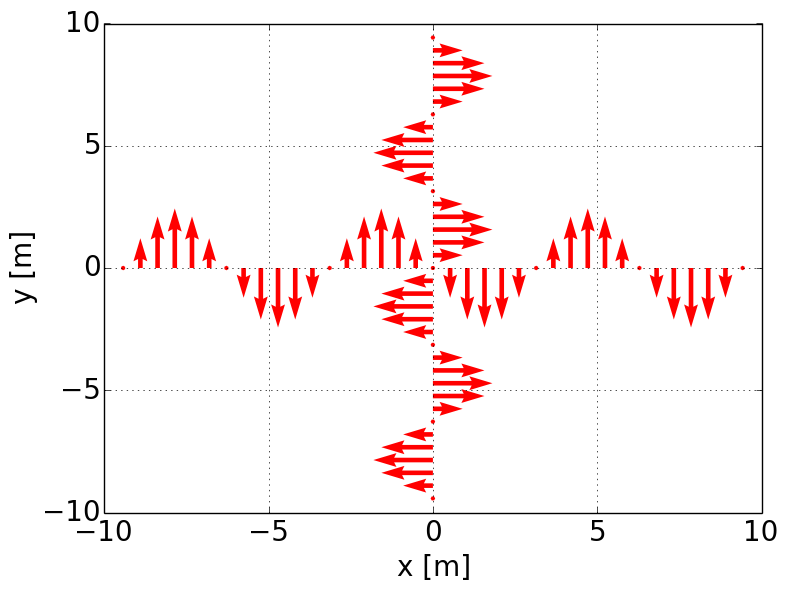
\includegraphics[width=0.7\linewidth]{../3b.png}
		\caption{Vektorene viser hvordan strømvektorene
        er langs x- og y-aksen. Dette er en sin-funksjon langs aksene.}
		\label{fig_3b}
\end{figure}



For å sjekke om figur \ref{fig_3b} er korrekt kan en se generelt
på hastighetsfeltet langs x-aksen og y-aksen:


\begin{align*}
    &\textbf{Langs x-aksen er $ y = 0$}
    &&\textbf{Langs y-aksen er $ x = 0$}
    \\
    &v_x = \cos(x)\sin(y) = 0
    &&v_x = \cos(x)\sin(y) = \sin(y)
    \\
    &v_y = - \sin(x)\cos(y) = -\sin(y)
    &&v_y = - \sin(x)\cos(y) = 0
\end{align*}

Dermed vet vi at vi burde få piler langs aksene som varierer
som en sin-kurve i størrelse.










\pagebreak
\subsection*{3 c)}

\textbf{Finn sirkulasjonen om randa til kvadratet
definert ved $-\frac{\pi}{2} \leq x \leq \frac{\pi}{2}$ og
$-\frac{\pi}{2} \leq y \leq \frac{\pi}{2}$.}
\\
\\
Vi vet fra GF at sirkulasjonen er definert som linjeintegralet
 over hastighetsfeltet. Vi deler opp integralet i 4 deler. En del for
 hver sideflate (starter ved nedre sideflate og beveger oss mot klokken):

\begin{align*}
    C =  \oint \mathbf{v} \dd r
    =
    \int_{a}^{b} \mathbf{v} \cdot \dd \mathbf{r}
    +
    \int_{b}^{c} \mathbf{v} \cdot \dd \mathbf{r}
    +
    \int_{c}^{d} \mathbf{v} \cdot \dd \mathbf{r}
    +
    \int_{d}^{a} \mathbf{v} \cdot \dd \mathbf{r}
\end{align*}

For a til b er $\dd \mathbf{r} = \dd x \mathbf{i}$.
For b til c er $\dd \mathbf{r} = \dd y \mathbf{j}$.
For c til d er $\dd \mathbf{r} = \dd x \mathbf{-i}$.
For d til a er $\dd \mathbf{r} = \dd y \mathbf{-j}$.
Dette gir oss følgende integraler og resultater:

\begin{align*}
    &\int_{a}^{b} \mathbf{v} \cdot \dd \mathbf{r}
    =
    \int_{-\frac{\pi}{2}}^{\frac{\pi}{2}}
    \mathbf{v} \cdot \dd x \mathbf{i}
    =
    \int_{-\frac{\pi}{2}}^{\frac{\pi}{2}}
    \cos(x)\sin(y) \dd x
    = 2 sin(y)
    \\
    &\int_{b}^{c} \mathbf{v} \cdot \dd \mathbf{r}
    =
    \int_{-\frac{\pi}{2}}^{\frac{\pi}{2}}
    \mathbf{v} \cdot \dd y \mathbf{j}
    =
    \int_{-\frac{\pi}{2}}^{\frac{\pi}{2}}
    - \sin(x)\cos(y) \dd y
    = -2\sin(x)
    \\
    &\int_{c}^{d} \mathbf{v} \cdot \dd \mathbf{r}
    =
    \int_{-\frac{\pi}{2}}^{\frac{\pi}{2}}
    \mathbf{v} \cdot \dd x \mathbf{-i}
    =
    \int_{-\frac{\pi}{2}}^{\frac{\pi}{2}}
    -\cos(x)\sin(y) \dd x
    = -2 \sin(y)
    \\
    &\int_{d}^{a} \mathbf{v} \cdot \dd \mathbf{r}
    =
    \int_{-\frac{\pi}{2}}^{\frac{\pi}{2}}
    \mathbf{v} \cdot \dd y \mathbf{-j}
    =
    \int_{-\frac{\pi}{2}}^{\frac{\pi}{2}}
    \sin(x)\cos(y) \dd y
    = 2 \sin(x)
    \\
    &\oint \mathbf{v} \dd r
    =
    2\sin(\frac{\pi}{2})
    + 2\sin(\frac{-\pi}{2})
    - 2\sin(\frac{\pi}{2})
    - 2\sin(\frac{-\pi}{2}) = -8
\end{align*}

 % Ved hjelp av Greens teorem får vi at
 % linje integralet er ekvivalent med flatearealet over virvlingen:

 % \begin{align*}
 %    C =  \oint \mathbf{v} \dd r
 %    =\int_{-\frac{\pi}{2}}^{\frac{\pi}{2}}
 %    \int_{-\frac{\pi}{2}}^{\frac{\pi}{2}}
 %    -2\cos(x)\cos(y)\textbf{k} \cdot \textbf{n} \mathbf{k}
 %    \qquad \dd x \dd y = 0
 % \end{align*}














\subsection*{3 d)}
\textbf{Forklar hvorfor det eksisterer en strømfunksjon for
feltet gitt i likning (1), se hintet i forrige oppgave.
 Vis at strømfunksjonen kan skrives }

 \begin{align}
    \psi = cos(x)cos(y)
 \end{align}

I hintene fra forrige oppgave står det at dersom et vektorfelt
er todimensjonalt i xy-planet, $\mathbf{v} = v_x \mathbf{i}
+ v_y \mathbf{j}$ og divergensfritt, $\partial v_x /\partial x
+  \partial v_y /\partial y = 0$, så eksisterer det en
 strømfunksjon som angitt ovenfor.
\\
\\
Ovenfor får vi definisjonen $v_x = \partial \psi /\partial y$
og $v_y = \partial \psi /\partial x$. Dermed er det bare å integre $v_x$
med hensyn på y og $v_y$ med hensyn på x.


\begin{align*}
    \int v_y \dd x
    &= \int - \sin(x)\cos(y) \dd x
    = \underline{\underline{\cos(x)\cos(y)}}
    \\
    - \int v_y \dd x
    &= - \int \cos(x)\sin(y) \dd x
    = \underline{\underline{\cos(x)\cos(y)}}
\end{align*}




















\pagebreak
\subsection*{3 e)}

\textbf{Bruk Taylorutvikling av andre orden til å
 finne tilnærmede strømlinjer nær origo.}


\begin{align*}
    &\psi(x,y) = T_2(\psi) + \mathcal{O}(x^3,y^3)
\end{align*}

Vi er kun interessert i $T_2(\psi)$ rundt origo:

\begin{align*}
    T_2(\psi)_{0,0} =
    &\psi(0,0)
    +
    \left(\frac{\partial \psi}{\partial x}\right)_{0,0} (x-0)
    +
    \left(\frac{\partial \psi}{\partial y}\right)_{0,0} (y-0)
    +
    \\
    &\frac{1}{2}
    \left(\frac{\partial^2 \psi}{\partial x^2}\right)_{0,0} (x-0)^2
    +
    \frac{1}{2}
    \left(\frac{\partial^2 \psi}{\partial y^2}\right)_{0,0} (y-0)^2
    +
    \left(\frac{\partial^2 \psi}{\partial x\partial y}\right)_{0,0} (x-0)(y-0)
    \\
    T_2(\psi)_{0,0} =
    &\cos(0)\cos(0)
    -\sin(0)\cos(0)x
    -\cos(0)\sin(0)y
    \\
    &-\frac{1}{2}
    \cos(0)\cos(0)x^2
    -
    \frac{1}{2}
    \cos(0)\cos(0)y^2
    +
    \sin(0)\sin(0)x^2
    \\
    \\
    T_2(\psi)_{0,0} =
    &\underline{\underline{
    1
    -\frac{1}{2}
    x^2
    -
    \frac{1}{2}
    y^2
    }}
\end{align*}





















%
